\chapter{September 2015}
        \section{September 1st, 2015}
    		Pinch and a punch for the first of the month!\\
    		
    		I played around with some more blender rendering today. Not much to report here. Did some more work on the website.\\
    		
    		I personally felt that the \index{regionals}regionals \index{routine}routine was much better than the \index{state}state one. I had given a few days to developing the regionals routine, and months of thought into songs and actions. I was able to take my relative time in putting a good routine together. I also felt that the \index{Christmas Tree}Christmas Tree prop provided a good "setting up" for the theme.\\
    		
    		In comparison, I spent 99\% of the time in preparation for States building the \index{stage}stage. Although I produced a very nice stage, I didn't find a good way to use it, so at 1AM on the night before the competition I was scrambling to get a routine that fit the stage usage. I made the routine fit the props, not the other way around.\\
    		
    		With these lessons learned, I have decided to do a little bit of routine development for a long period of time (30min or more a day for a month). This will allow me to look into getting a great selection of music that flows together well in a flowing story. I have time to remove or change parts of the routine if I need to.\\
            
            \textit{\textbf{Also see: }\hyperref[Props]{Props}}
    		
    		After talking to people, and reviewing the footage I have noticed that using popular \index{songs}songs that everyone knows generally draws in the audience. As such, I have tried to continue this \index{theme}theme. Here is a \index{screenshot} of my \index{brainstorming}brainstorming \index{spreadsheet}spreadsheet as it stands:\\
    		
    		\centerline{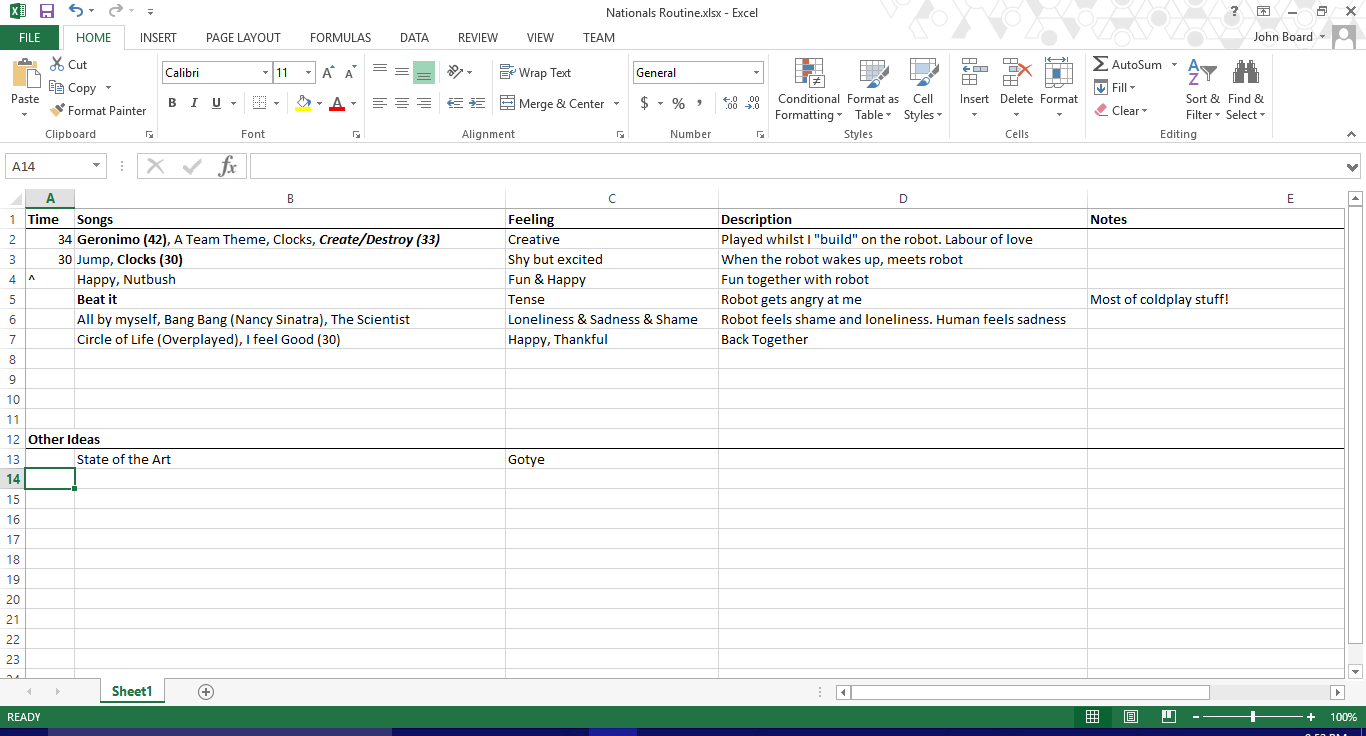
\includegraphics[width=\linewidth]{images/Songs}}
    		\vspace{10pt}
    		
    		I'm a great believer in \index{story telling}story telling. I wanted to convey a flowing emotion throughout the performance. I believe this draws the audience in, and can evoke an emotional feeling in them. For this routine I \index{modeled}modeled the story off a Biblical Parable, "The Prodigal Son".
            
            \textit{\textbf{Also see: }\hyperref[Story]{Story}}
    		
    		I'm now fairly happy with the selection of \index{songs}songs - and I'm getting excited about the routine. I think it'll be the best one yet. (or maybe it's just because I'm tired, it's 12:11AM - can't get to sleep).\\
    		
    		I've started cutting the songs together using \index{Audacity}Audacity. I've just cut together the snipping of sound from \textit{"Create/Destroy" - Art vs Science}. When \hyperref[audio_editing]{editing} the songs together I have to be careful about where I cut the music of them. If you cut a track in the wrong place it can sound disjointed.\\
            
            \index{audio editing}
            \index{cutting audio}
            
            \textit{\textbf{Also see: }\hyperref[audio_editing]{Audio Editing}}
    		
    		I use a few tricks to get around this. Firstly (and the one that seems to make the most sense), I fade the tracks in and out (and sometimes into each other). The second trick, and one that I've used twice now with great success, is to cut the start and the end of a song together. The best example of this is \textit{"I Feel Good" - James Brown}, in the regional and state routines where I took the starting section "Heeeeyyy! I feel good, nanana...", and stitched it to the end, "so good (bump bump), so good (bump bump), I got a-you....". I'm also using this trick with the \textit{Create/Destroy} sound track as I've found that cutting the sound track part way through doesn't sound good, but if I stitch the start and end together carefully, it sounds much better as the song naturally ends.\\
    		
    	\section{September 2nd, 2015}
    		Today I've been working on the website. I think it looks quite spiffy now. I'm using the \index{Wordpress}wordpress theme, \index{Enigma}Enigma. The website is designed to provide a portfolio for what I do, and place which I can share information and things that I've learnt. It can be found at:\\
    		
    		\url{http://johnrobboard.com/}\\
    		
    		I ran the design by a few people on Facebook, and got a positive response, with some suggestions which I've now implemented.\\
    		
    		I've also been finalizing the \index{songs}songs for my \index{nationals}nationals routine. I've swapped out \textit{"All by myself"} for \textit{"Bang Bang"} - Nancy Sinatra. I came to this conclusion after consistent disgust with \textit{"All by myself"}. I felt \textit{"Bang Bang"} is a very good match for the routine as it seems to even narrate the story. During the song it says "he wore black, and I wore white...", as the \index{hexapod}hexapod is black, I was thinking I could wear a white \index{lab coat}lab coat. This would fit in quite nicely.\\
    		
    	\section{September 3rd, 2015}
    		Today has been quite stressful as I've been organizing my QTAC applications and SAT exam dates. I only get one shot at the SAT exam, and it's only a week after Nationals. I'm going to have to fit robocup into a tight study schedule.\\
    		
    		I would like to more or less finalize the music in the next few days, which will allow me to start animating in plenty of time, as to not stress my SAT prep. I have enough time to do everything, if I'm wise as to how I spend it.\\
    		
    		Currently I'm looking at using:\\	
    		
    		\begin{enumerate}
    			\item{Create/Destroy - Art vs. Science}
    			\item{Clocks - Coldplay}
    			\item{Beat it - Michael Jackson}
    			\item{Bang Bang - Nancy Sinatra}
    			\item{Circle of Life - The Lion King}
    		\end{enumerate}
            
            \textit{\textbf{Also see: }\hyperref[audio_selection]{Song Selection}}
    		
    		I think there's possibly a better song than Circle of Life for the ending, but haven't found it yet. The key is fitting in all of these songs. I might cut short Create/Destroy.\\
    		
    		I'm also looking at getting back into my army fitness training, as there are a few events next month which I'll need my fitness up for again.\\
    		
    		To organize my time I use a method by Dr. Stephen Covey in his book, \textit{"The Seven Habits of Highly Effective People"}. This has helped me organize my time significantly, and I have seen great improvement because of it - and the other habits he outlines in his book.\\
    		
    	\section{September 11th, 2015}
    		It's been many days since I've worked on anything important, and this is mainly due to the demise of the monitor on my old laptop. The hinges holding the monitor onto the base of the laptop had separated from the base. Although fixable in the short term, I'll be needing a working laptop for Uni next year, so I opted to purchase a new one. I ended up acquiring a Razer Blade 14".\\
    		
    		As for the old laptop, it's electronics still work very suitably, so I opted to turn it into a "porta-desktop". I didn't want to leave the \index{monitor}monitor on it because I felt leaving a half broken monitor had a chance of damaging the base even further. I removed it, and now use it with one of my many unused external monitors.\\
    		
    		There were also a few minor issues with the laptop, such as a very dodgy \index{power jack} \index{jack}power jack, broken audio jack, and 2 broken USB ports. Whilst I had the laptop open to take the monitor off I fixed these problems through soldering, etc. The "surgery" went well, and my sister is now using it.\\
    		
    		\centerline{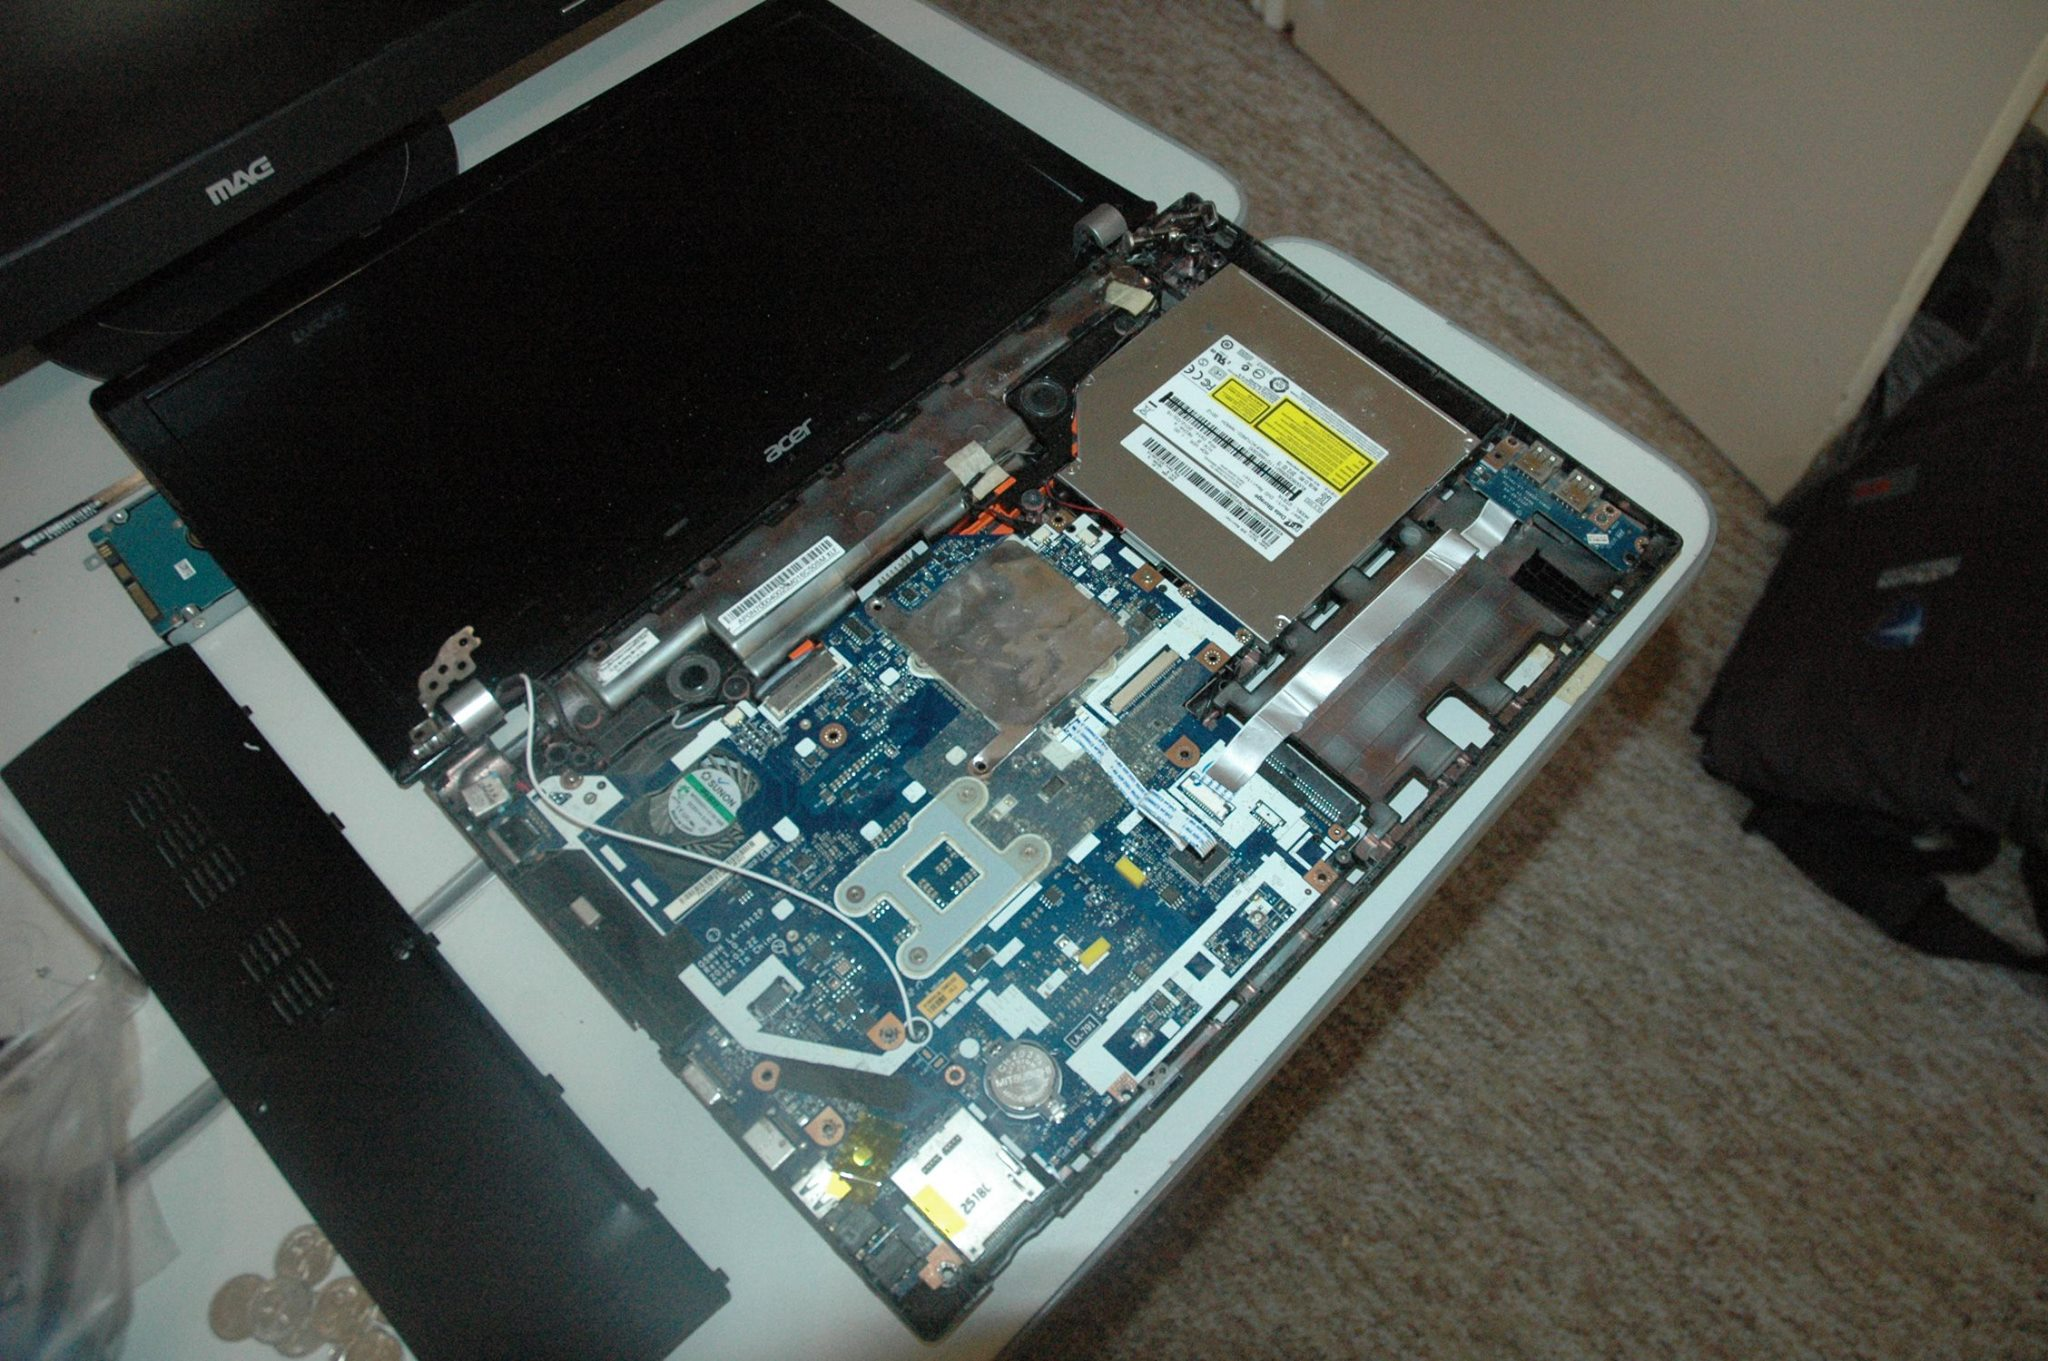
\includegraphics[width=\linewidth]{images/laptop_repair_1}}
    		\vspace{10pt}
    		
    		\centerline{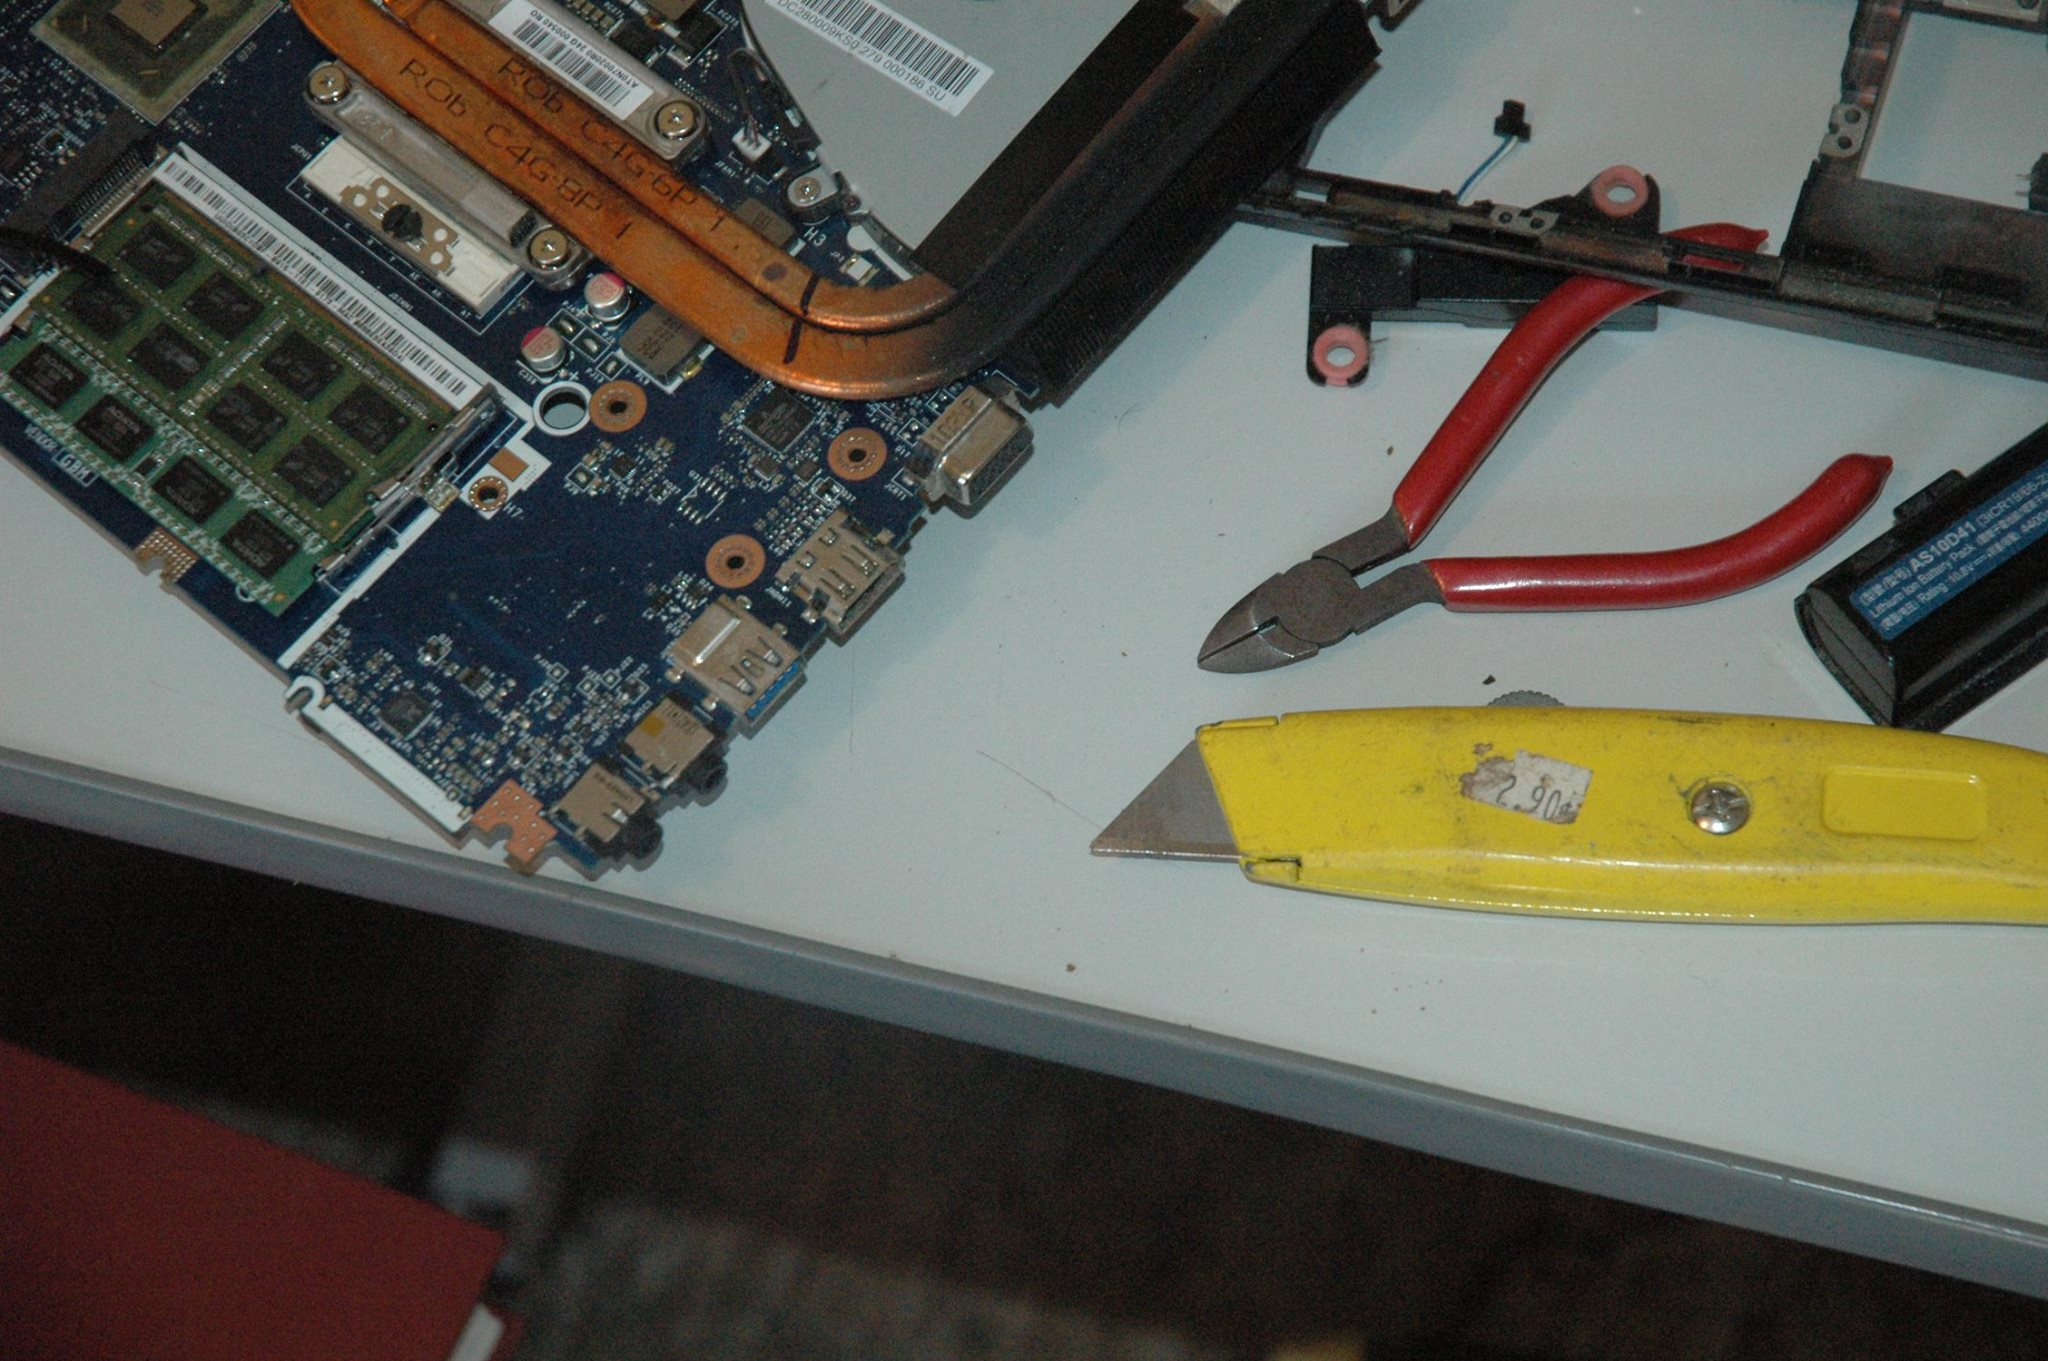
\includegraphics[width=\linewidth]{images/laptop_repair_2}}
    		\vspace{10pt}
    		
    		\centerline{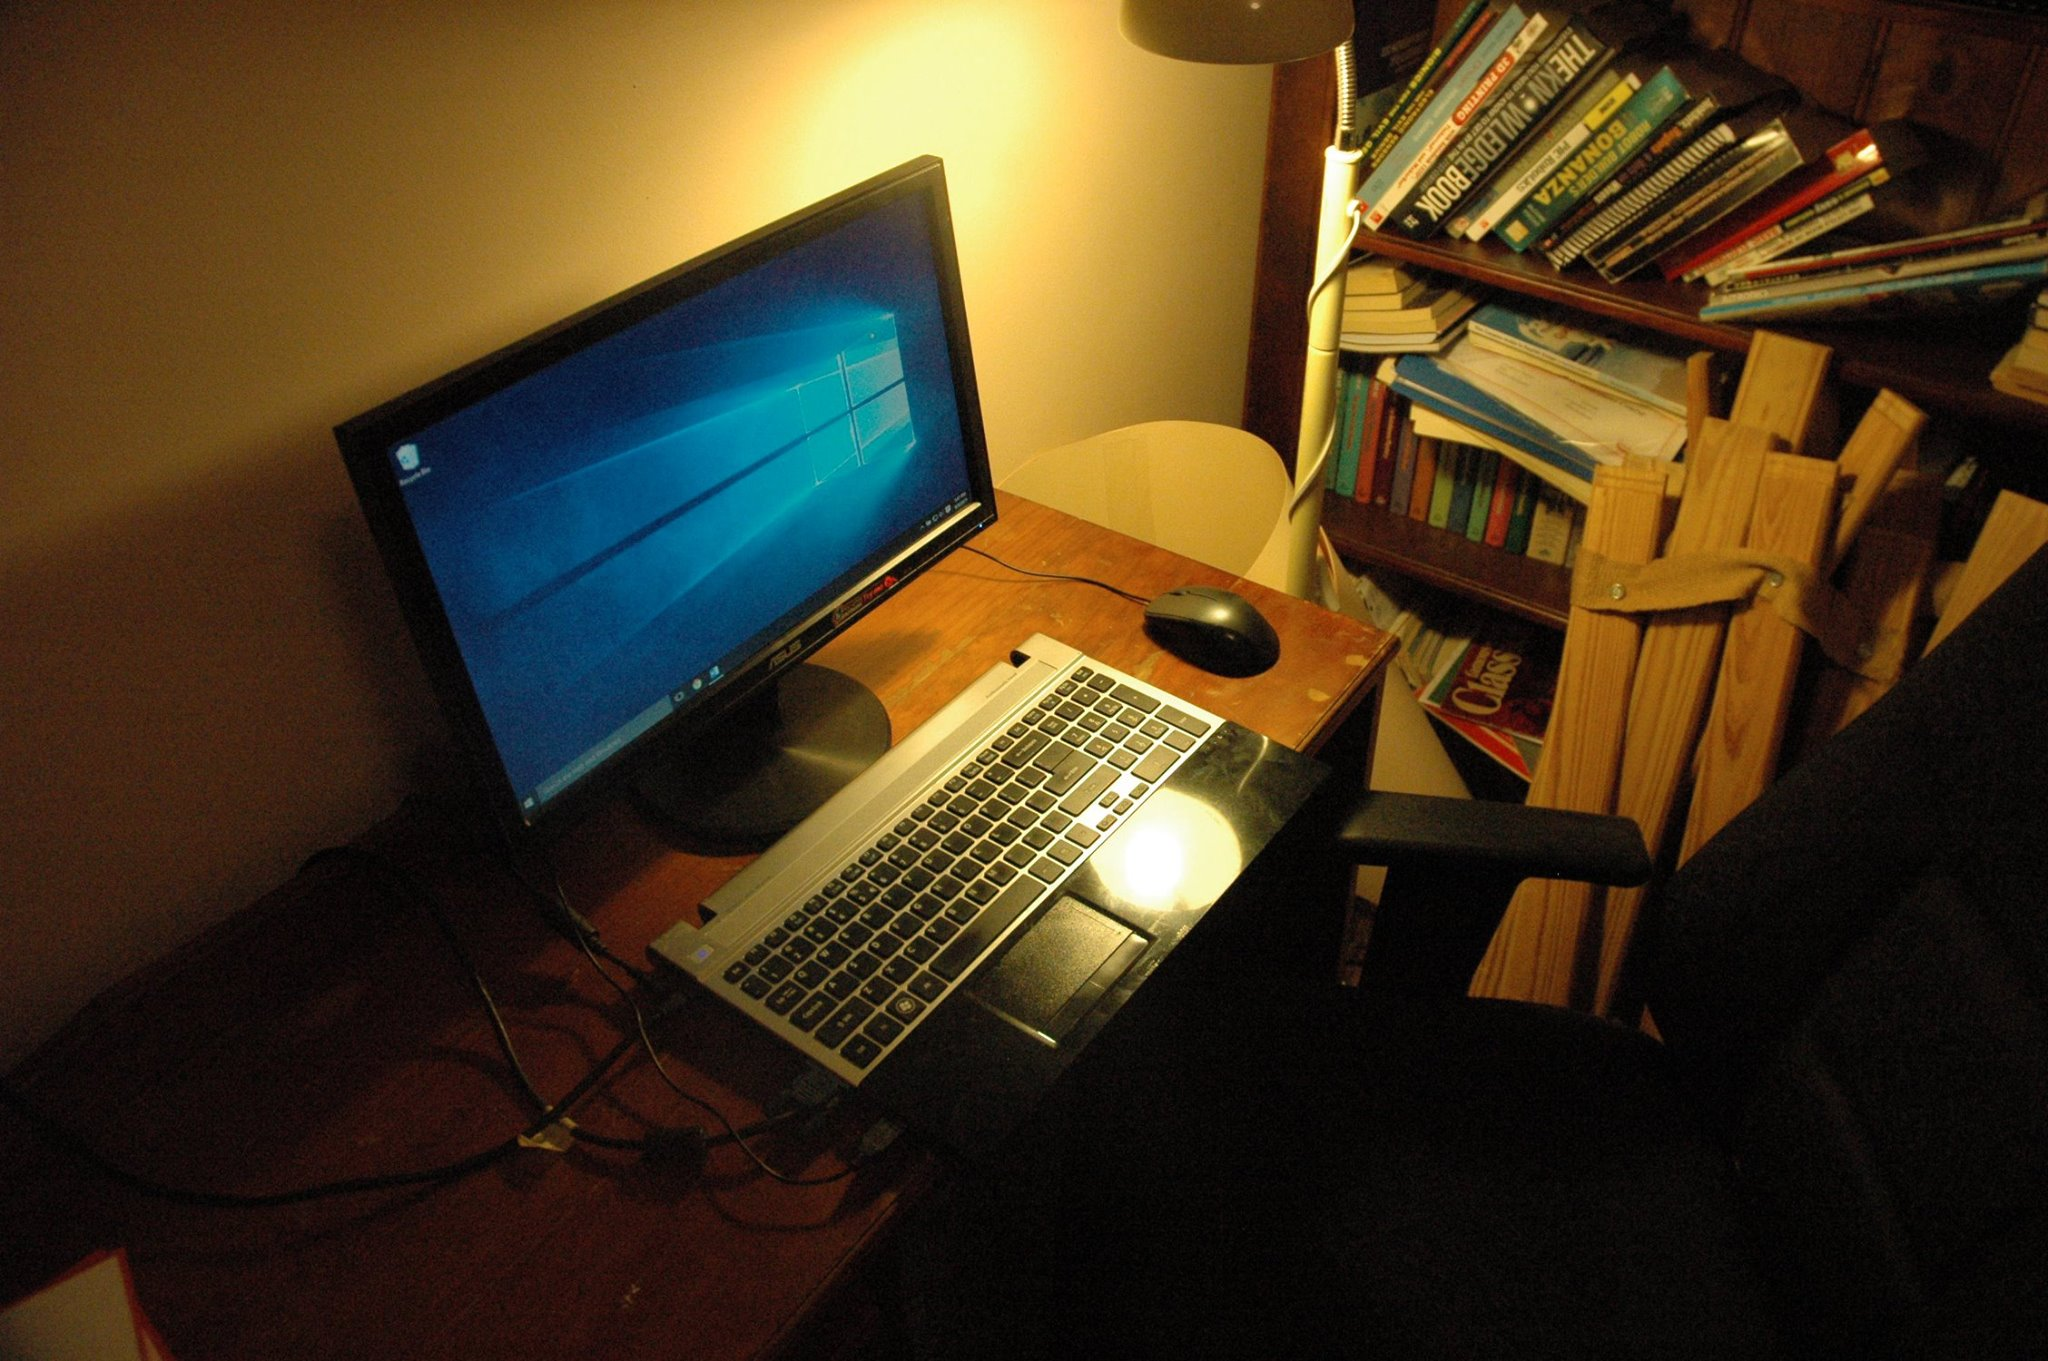
\includegraphics[width=\linewidth]{images/laptop_repair_3}}
    		\vspace{10pt}
    		
    		After the laptop fiasco, I went back to setting up my new laptop. I save all my files for this project on \index{BitBucket}BitBucket (due to free private hosting, compared to using GitHub). I tried git cloning the project onto my laptop and was annoyed to find out that it didn't work - over both HTTP and SSH cloning. It would fail at 8\% (which took ~15min to reach), because of some error.\\
    		
    		I finally decided to download it directly as a zip from my \index{BitBucket} account. I was surprised to find it was some 600MB in size. After attempting to download it multiple times, I was disappointed to find my download speed never went above 100KB/s. I had previously been playing around with \index{VPS}\index{hosting}VPS/Web hosting services to get my website a little closer to home (to allow for faster download speed and less latency). I had played around with using an \index{Amazon}\index{EC2}Amazon EC2 instance, and still had my account set up. I remembered that I had noted that the EC2 instances had fantastic internet speeds, so I launched an instance of \index{Linux}\index{Ubuntu}Ubuntu 14.04, from which I \index{wget}wget'ted the zip (using \index{HTTP}HTTP auth) from BitBucket. This process took less than ~3min, achieving a peak speed of 7.4MB/s. I then downloaded from that host onto my computer achieving a peak speed of 4.2MB/s (obviously much faster than 100KB/s). This process was very satisfactory, and was completed in under 10min (compared to a prospective hour or more).\\
    		
    		I downloaded the \index{Adobe Creative Cloud}\index{Adobe}Adobe Creative Cloud onto my computer, with a view of trialling such software as Premiere, After Effects, \index{Photoshop}Photoshop, Illustrator, but more specifically for RoboCup - Audition (the sound editing software). I'm using the 30 day trial, but leaving money aside should I wish to purchase a year subscription to the student creative cloud.\\
    		
    		I also installed the student versions of \index{Autodesk}\index{Maya}Autodesk Maya, and have the intention to install others from the Adobe suite.\\
    		
    		I have been pleasantly surprised by how much I've been enjoying the graphical design aspects of \index{Blender}Blender. I've been getting an appreciation of what graphics designers do. I'm considering spending some significant time each week learning how to use the professional tools such as Photoshop, Premiere, Audition, Maya, and Blender over the next few years. I believe this will enhance my skillset and help me become a more well rounded engineer.\\
    		
    		I've had many people suggest in the past that I should start up a YouTube channel about the stuff I do. I have considered this proposal, and am willing to purchase a video camera as finances allow. This also contributes to my want to learn how to use After Effects and Premiere.\\
    		
    		In an attempt to further my documentation I downloaded a program that takes \index{screenshot}screenshots every 5 seconds, and stores them. I did this with a view to creating a stop motion of me animating the robot. This will hopefully give people an idea of what goes into me programming my robot. I have run this process, and captured some 7000 frames. I will stitch these together in the appropriate software when the time permits. I will upload this to YouTube.\\
    		
    		Currently the code that I've written for extracting movements from Blender works, but it can be improved. Namely, because I couldn't originally figure out how to extract bone rotations from the Animation UI from \index{Blender}Blender, I had to animate the routine, and then play it back in the Blender \index{Game Engine}Game Engine. This is quite suboptimal, and as such today I researched into getting the bone rotation information straight from the Animation UI. I asked around on the \index{Blender}Blender \index{python}python \index{API}API \index{IRC}IRC channel. I struck up a conversation with a very helpful gentleman...\\
    		
            \index{Blender development}
            \index{Blender scripting}
            \index{scripting}
    		\centerline{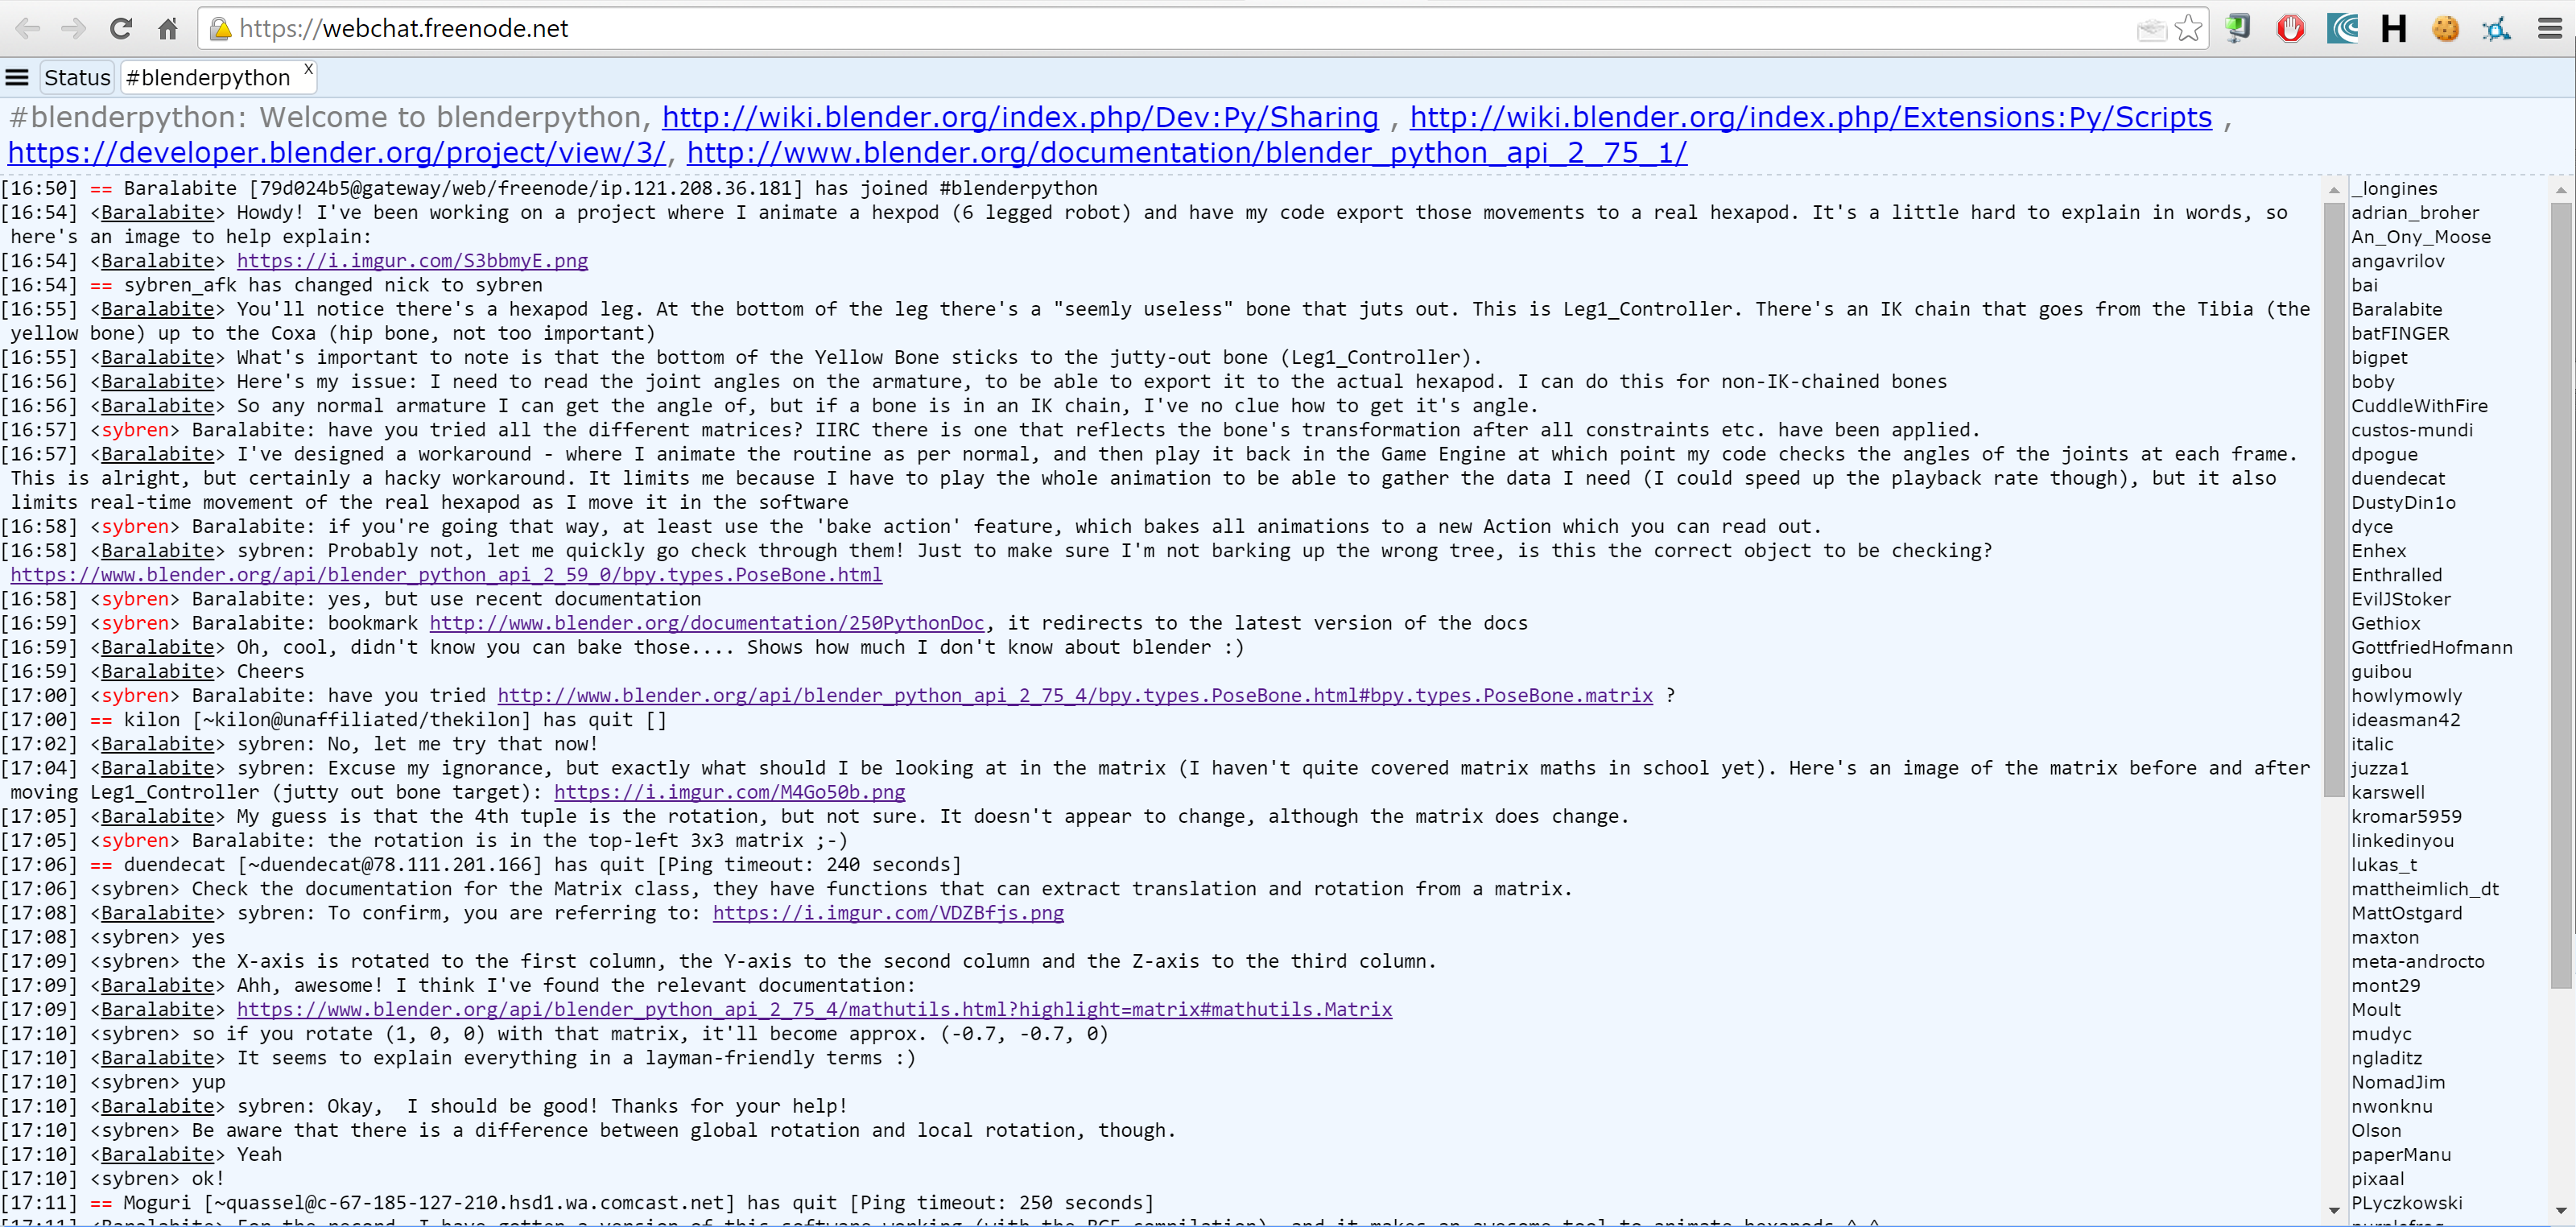
\includegraphics[width=\linewidth]{images/blender_irc}}
    		\vspace{10pt}
    		
    		This lead me to writing the following code:
    		
    		\centerline{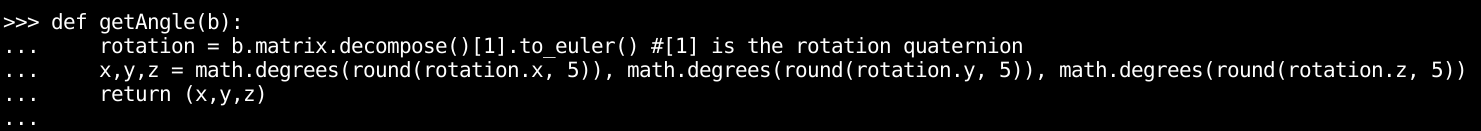
\includegraphics[width=\linewidth]{images/matrix_rotation_extractor}}
    		\vspace{10pt}
    		
    		This code returns an \index{euler}Euler XYZ tuple of the rotation values in degrees, very similar to the one I got from my Game Engine code.\\
    		
    		The advantage of getting the \index{rotation}rotation values in this way is that I can now have the \index{robot}robot respond in real time to moving the robot around on screen. In other words, I can move the robot around on screen, and have it do that in real life. This is as opposed to having to compile the animation, ship it to the game engine, replay it - gather the rotation values while it's replaying, etc. Also this feature will speed up the time it takes from finishing \index{animation}\index{animating}animating the routine, to testing it on the robot in the order of magnitudes.\\
    		
    	\section{September 12th, 2015}
    		Today I've been working on finalizing the routine music. I've decided not to use \textit{"Bang Bang" - Nancy Sinatra} in lieu of going back to \textit{All by Myself - Celine Dion}. The reasoning behind this is that I wanted distinct sections in the routine where the robot shooed me (Beat it), and more importantly a good section where we feel sorrowful for being apart, and want to come back together. Bang Bang was excellent for prompting sorrow, but I would need another song for "getting back together", whereas All by Myself has this "built in" - it has a sorrowful part, and then a getting back together part. I chose this because of time restrictions.\\            
    		
    		I've switched from using \index{Audacity}Audacity to using \index{Adobe}Adobe Audition (30 day trial). I've really enjoyed learning how to use a new tool. Audition's quality is outstanding, and I look forward to using it in the future. I've finally settled on the audio I want to use.\\
    		
    		I'm also going to install \index{Rasbian}\index{Linux}\index{Debian}Rasbian on a \index{RPi}\index{Raspberry Pi}RPi tonight. Hoping to "upgrade" the old brain to this new one while I'm improving software and electrical systems. When I say upgrading, I'm going from RPi B to RPi v2.\\
            
            \textit{\textbf{Also see: }\hyperref[Rasberry Pi]{RPi}}
    		
    		On a completely separate note I've been preparing for a talk I'm giving in December at a camp. I've been thinking about what I want to talk about. Through thinking about the talk I've been trying to figure out why I procrastinate tasks. I'm not satisfied with the answer, but I think I procrastinate because I have fear of "the unknown". If I commit to completing a task, I don't know how it'll turn out. If I pretend the task doesn't exist, "maybe it'll go away" (which I realize is completely rubbish). I think the best way to combat this is by realizing that I can learn just as much from failure than from success - and that the time commit to a worthwhile task (no matter the consequence) will yield greater results than wasting time on Facebook, or watching movies.\\
    		
    		I don't think that's what I'll talk about though, I haven't had enough experience on it to talk about it. Instead, I've been looking at talking about humility. A lot of the guys coming on the camp are a little younger than myself, but are up and coming (aspiring) leaders. I'm thinking of talking about humility. Although I'm far from a humble person, I think I might have more to talk about than procrastination - I have much experience at being proud, and it's destructive properties. RoboCup has caused me to be very proud - and has humbled me as well. I'm inspired by humility in leaders, and I seek to achieve the same. Humility is the key to wisdom and knowledge.\\
    		
    		In other news, I've downloaded the latest stable Raspbian image (05-05-2015), and in the process of writing it to the SD card via \index{Win32DiskImager}\index{SD Card}Win32DiskImager. Whilst looking at card readers(/writers) for my new laptop, I decided to go with a USB 3.0 option with the hopes of getting faster write speeds. From past experience I know that writing to the 32GB SD cards can take a while, and without researching it I was guessing that USB 2.0 may have been bottle-necking the procedure.\\
    		
    		I'm going to record the speed it takes to write the Raspbian image to a 32GB disk. Time taken was 3min 47sec. Min transfer speed was 12.5MB/s, max transfer speed was 14.7MB/s, and average transfer speed was 13.5MB/s. As I didn't record speeds for a USB2.0 reader, I have no comparison. I may test this in the future.\\
    		
    		I'm attempting to boot up the RPi v2, and having difficulty getting both HDMI and Composite output. I'm going to logging in via SSH. To find out it's IP I scan the network using \index{port scanner}\index{scanner}\index{Advanced Port Scanner}\textit{Advanced Port Scanner}. Without this software, there are two options. One is manually pinging computers, secondly logging into the network gateway/DHCP server and check recent \index{DHCP}DHCP lease.\\
    		
    		\centerline{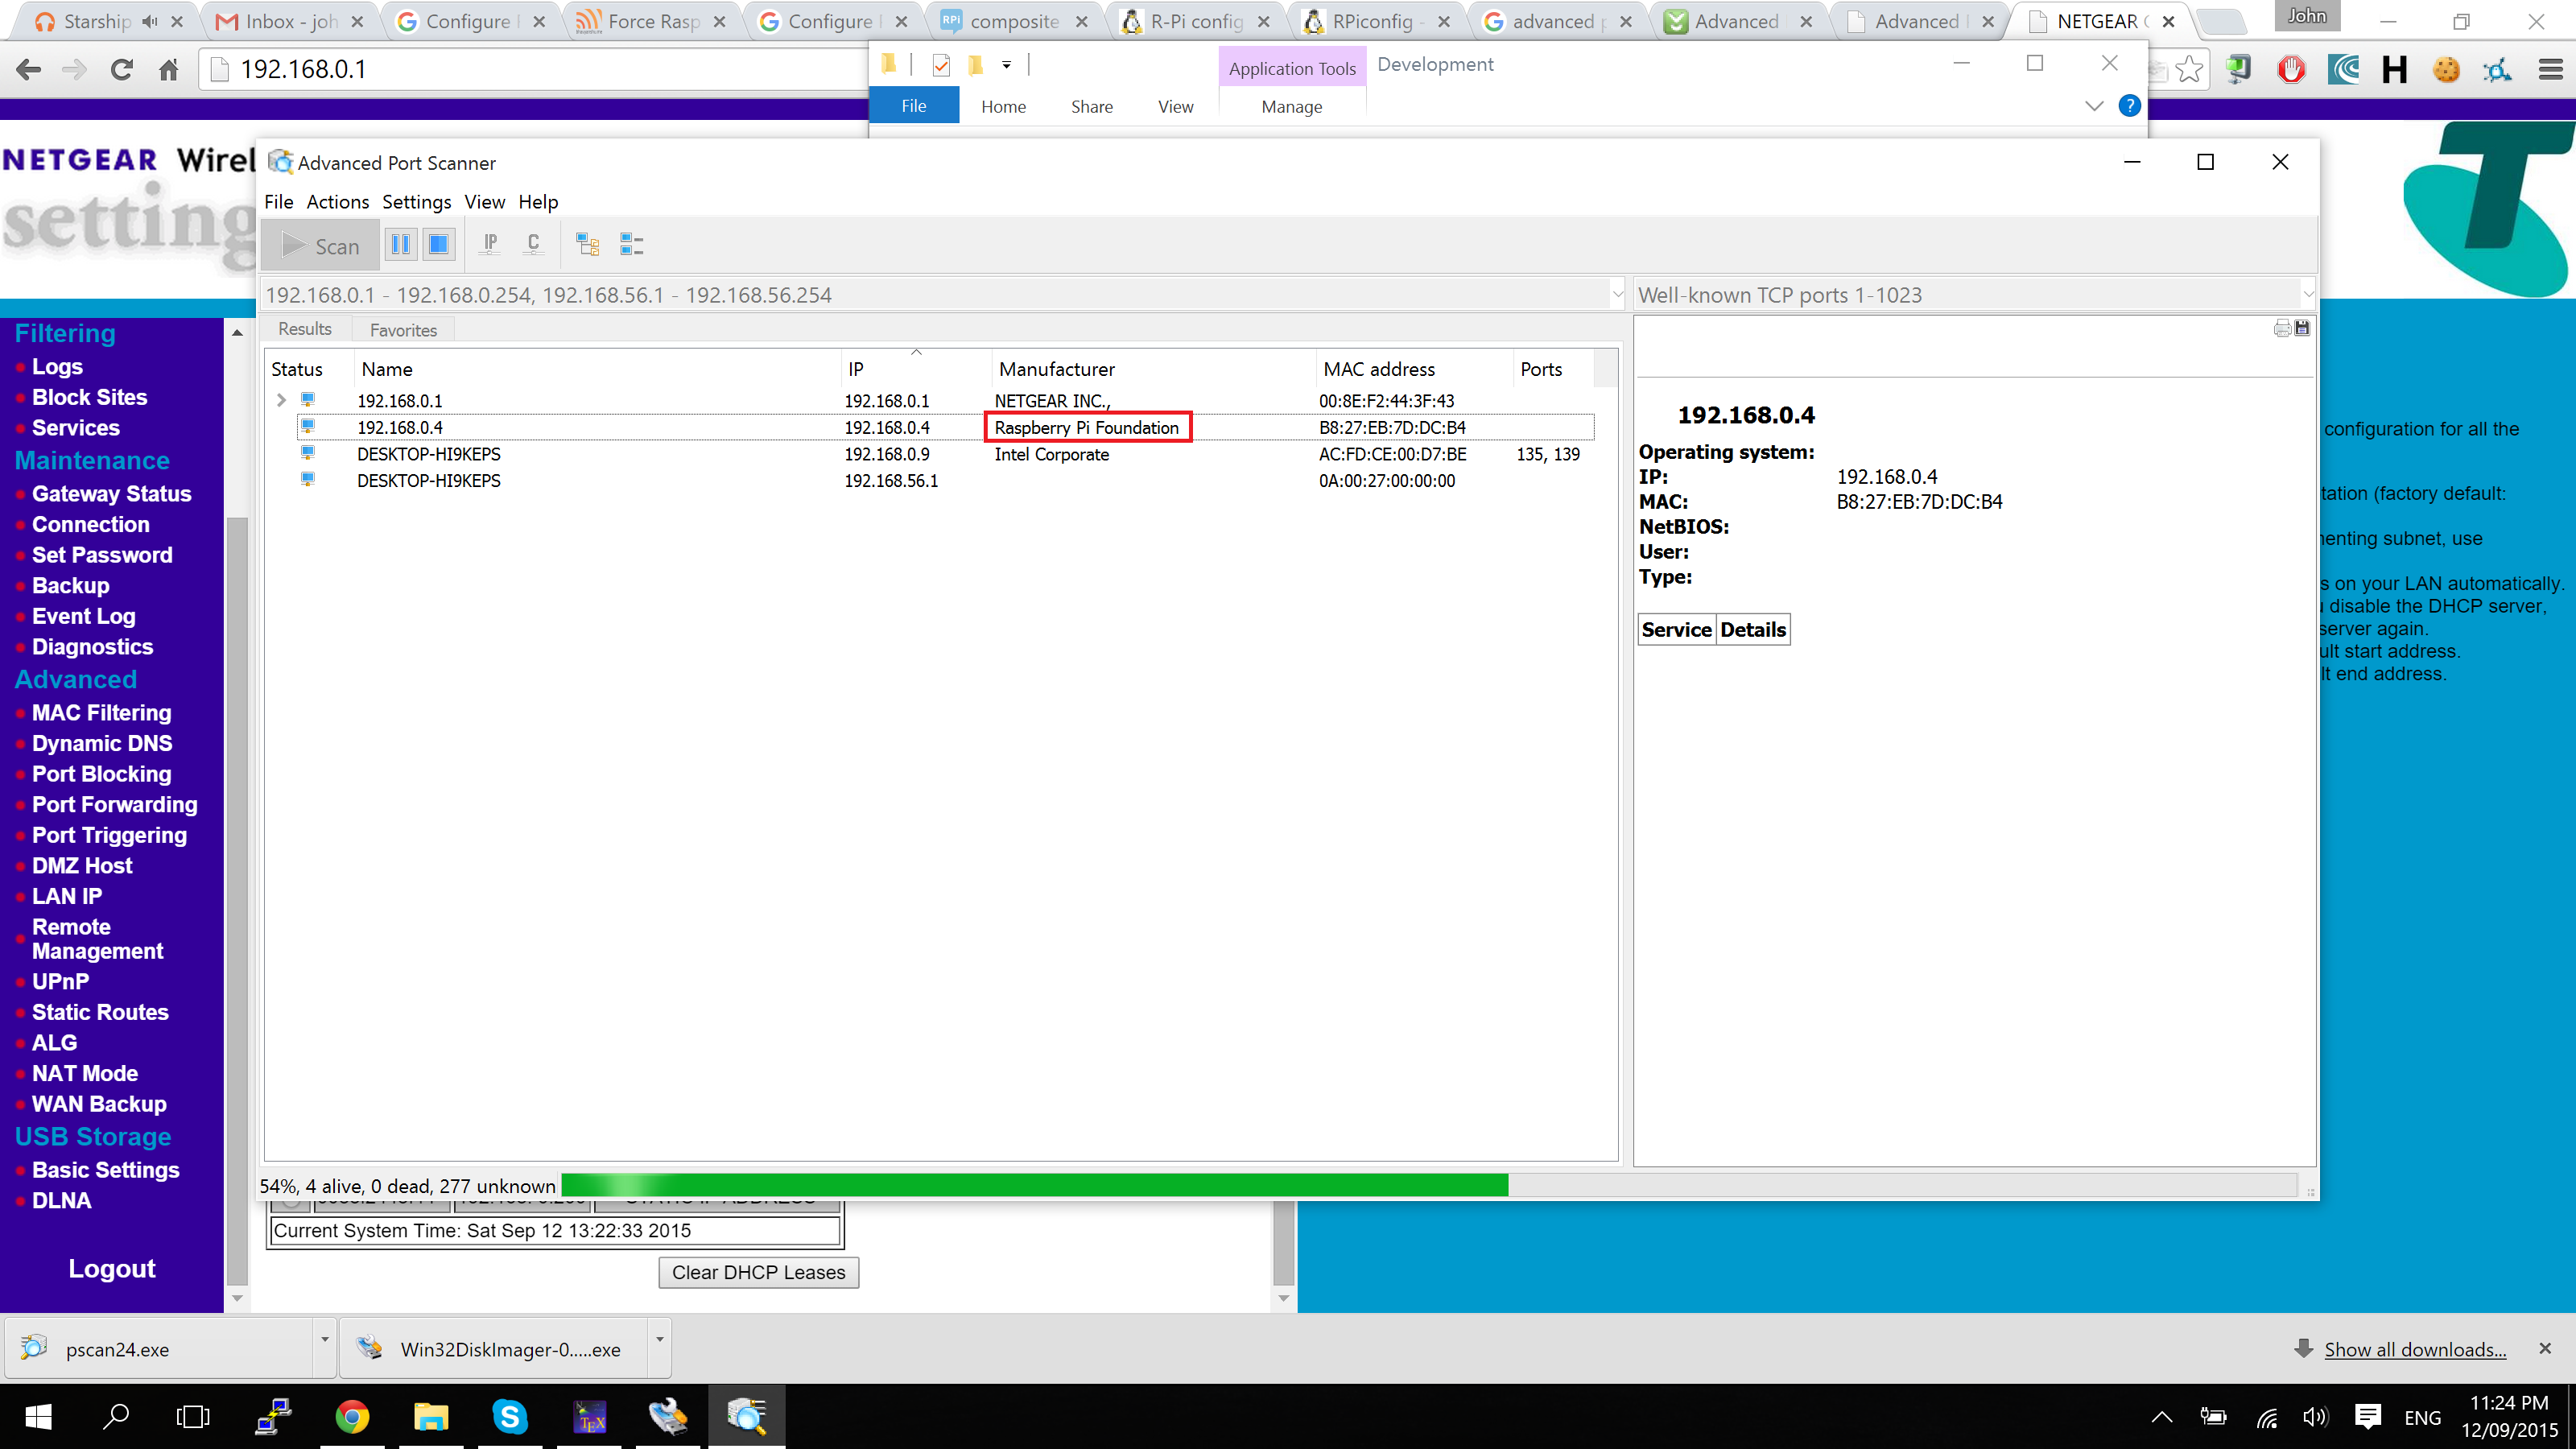
\includegraphics[width=\linewidth]{images/port_scanner}}
    		\vspace{10pt}
    		
    		And we're in! Firstly I run the raspi-config command, which allows me to set some settings like \index{SSH}SSH, \index{password}passwords, but most importantly it lets me change the partition to house the entire disk.\\\index{login}
    		
    		\centerline{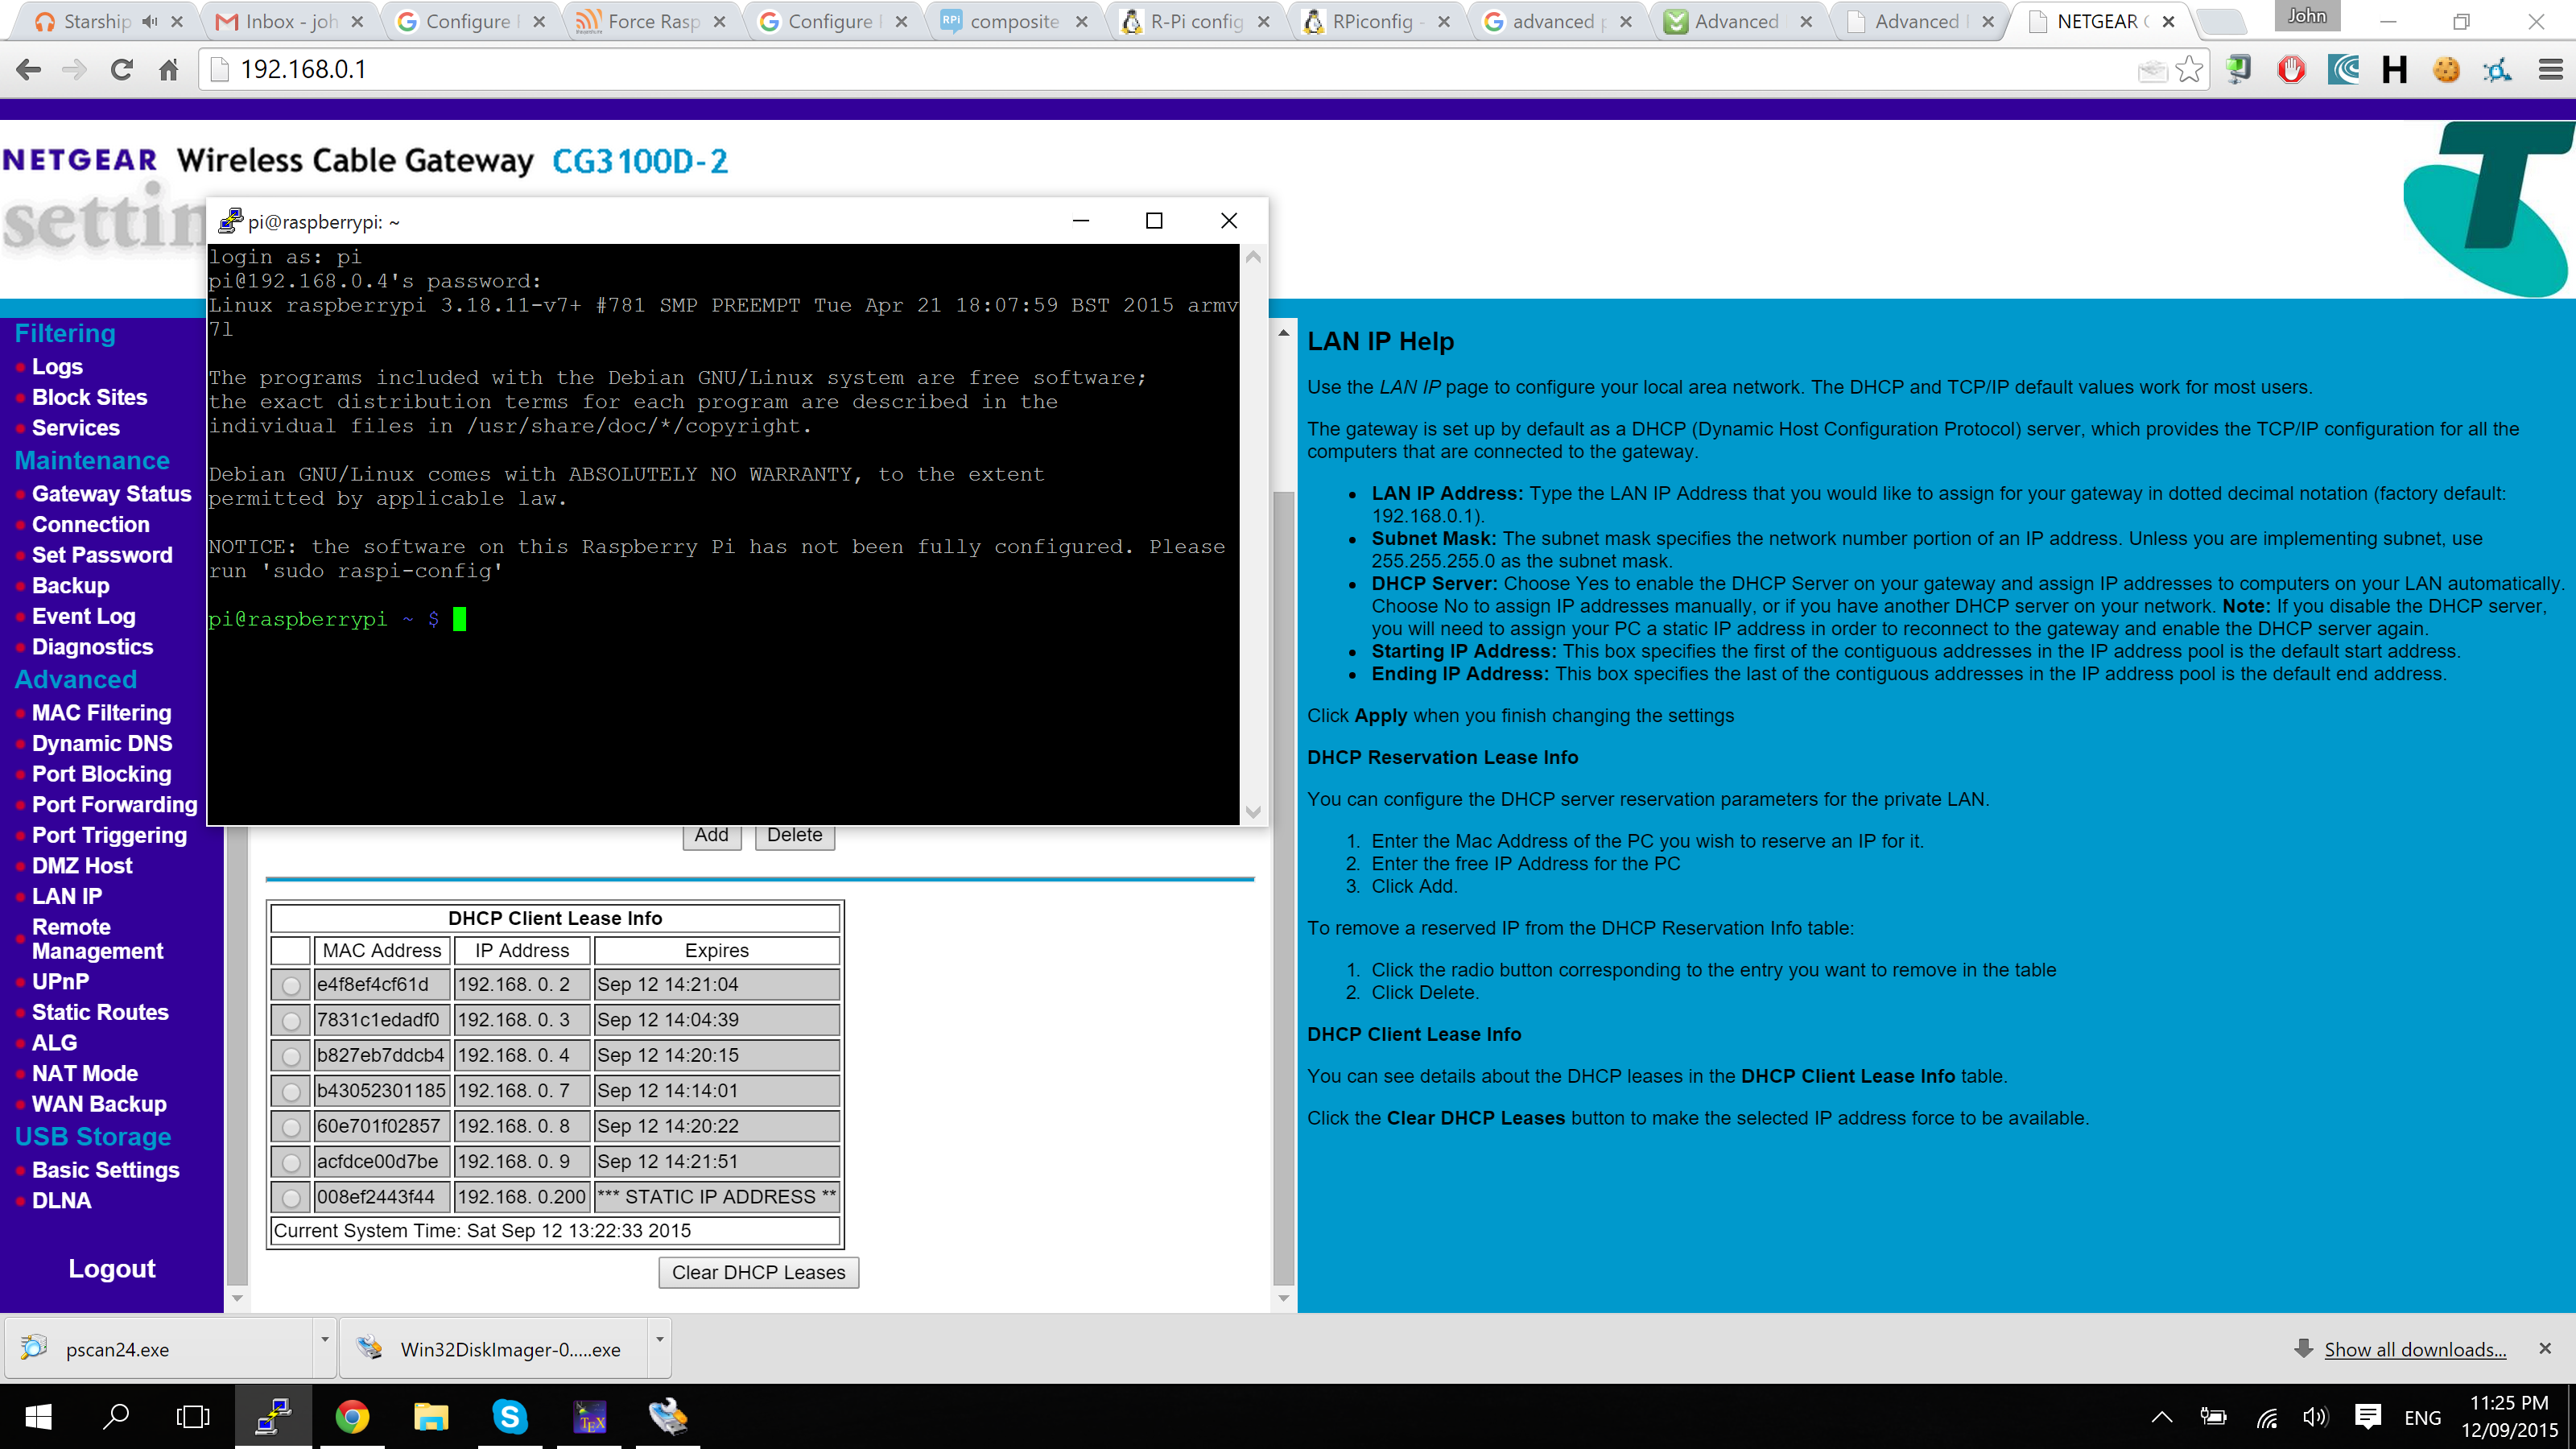
\includegraphics[width=\linewidth]{images/ssh_login}}
    		\vspace{10pt}
    		
    		For now I'll ditch trying to get \index{monitor}\index{HDMI}\index{composite}HDMI/Composite output, I don't generally intend to have anything but the \index{CLI}CLI running on the RPi monitor out because of the intense resource usage, and general uselessness of it.\\
    		
    		I now need to configure the RPi install to what I need. More details about this are outlined in the \hyperref[raspbian_install]{Software chapter} of the \hyperref[part:part_six]{BaralabaBob Technical Manual}.\\
            
                		
    		This process typically includes me setting a static IP for the network interface, thus allowing me to use the RPi without a DHCP server (because I can just configure my network interface on my computer to the correct subnet manually.).I also install the software I use (generally just \index{git}, \index{python}, screen, and \index{htop}).\\
            
			\textit{\textbf{Also see: }\hyperref[rpi_networking]{Networking}}                        
    		
    		I got slightly distracted when I realized that I was using the old LaTeX coding convention (aka, none) in the \hyperref[part:part_six]{BaralabaBob Technical Manual}, so I updated to the current standard that I use.\\